\begin{exercise}
      {ID-cd6ac26505aaa68d1570175c5645e808e33ac82f}
      {Unendlich viele Dreiecke}
  \newcommand{\topdowntriangle}[3]
  {%
    % zeichne ein graues, auf dem Kopf stehendes, gleichseitiges Dreieck
    \filldraw[fill=black!40!white] (#1, #2) -- ++(60:#3) -- ++(180:#3) -- cycle;
  }%
  \ifproblem\problem\par
    Die folgende Abbildung zeigt gleichseitige Dreiecke. Das größte (äußere) Dreieck
    besitzt den Flächeninhalt 1.
    \begin{center}
      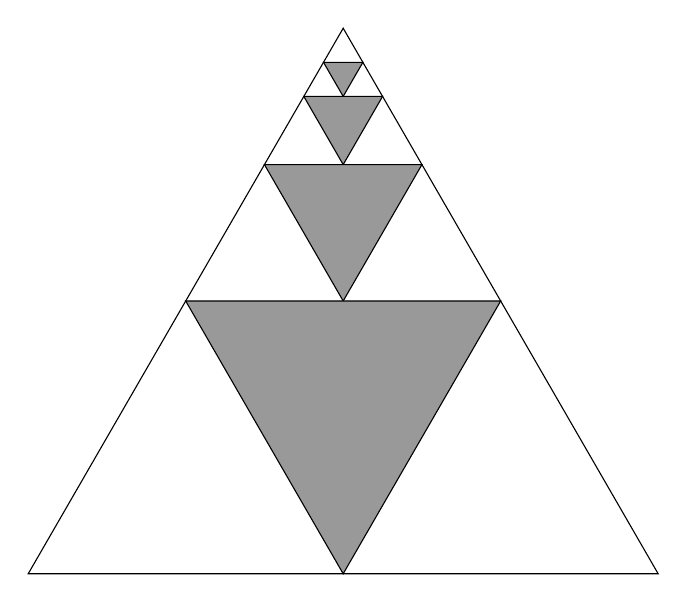
\begin{tikzpicture}[scale=0.5]
        \topdowntriangle{0}{12.12435}{1};
        \topdowntriangle{0}{10.3923}{2};
        \topdowntriangle{0}{6.9282}{4};
        \topdowntriangle{0}{0}{8};
        \draw (-8, 0) -- (8, 0) -- ++(120:16) -- cycle;
      \end{tikzpicture}
    \end{center}
    \begin{enumerate}[a)]
      \item Berechne den gemeinsamen Flächeninhalt der 4 grauen Dreiecke.
      \item Angenommen, man setzt die Konstruktion der grauen Dreiecke
            unendlich oft nach oben in die Spitze des äußeren Dreiecks fort.
            Wie groß wird dann die gemeinsame graue Fläche letztendlich werden?
    \end{enumerate}
  \fi
  \ifoutline\outline\par
    Vielleicht hilft es, wenn man in \textit{Trapezen} denkt statt in \textit{Dreiecken}\ldots
  \fi
  \ifoutcome\outcome\par
    Letztendlich beträgt der Flächeninhat der grau gefärbten Fläche $\frac{1}{3}$.
    Drei benachbarte Dreiecke bilden in jeder \glqq Reihe\grqq{} ein Trapez.
    Von jedem dieser Trapeze ist ein Drittel grau gefärbt, also ist letztendlich
    auch ein Drittel des großen Dreiecks grau gefärbt.
  \fi
\end{exercise}
